\documentclass[11pt,xcolor=dvipsnames]{beamer}
\usetheme{Warsaw}
\usepackage[utf8]{inputenc}
\usepackage[french]{babel}
\usepackage[T1]{fontenc}
\usepackage{amsmath}
\usepackage{amsfonts}
\usepackage{amssymb}
\usepackage{graphicx}

\definecolor{Vert}{RGB}{116,185,44}
\definecolor{Bleu}{RGB}{31,29,108}


\setbeamercolor{frametitle}{bg=Vert}
\setbeamercolor{framenumber}{bg=Bleu,fg=white}
\setbeamerfont{page number in head/foot}{size=\large}
\setbeamercolor{structure}{fg=Vert!90!black}

\setbeamertemplate{footline} {
  \leavevmode%
  \hbox{%
  \begin{beamercolorbox}[wd=.4\paperwidth,ht=2.25ex,dp=1ex,center]{author in head/foot}%
    \usebeamerfont{author in head/foot}\insertshortauthor
  \end{beamercolorbox}%
  \begin{beamercolorbox}[wd=.5\paperwidth,ht=2.25ex,dp=1ex,center]{title in head/foot}%
    \usebeamerfont{title in head/foot}\insertshorttitle\hspace*{3em}
  \end{beamercolorbox}}%
  \begin{beamercolorbox}[wd=.1\paperwidth,ht=2.25ex,dp=1ex,center]{framenumber}
     \usebeamerfont{framenumber}\insertframenumber{} / \inserttotalframenumber\hspace*{1ex}
  \end{beamercolorbox}%
  \vskip0pt%
}

\pgfdeclareimage[height=0.6cm]{logo}{../img/paquito.png}
\logo{\pgfuseimage{logo}}

\author{Paquiteam}
\title{Préesentation des cas d'utilisation principaux}
\subtitle{Paquito, easy packaging}


\date{26 janvier 2016} 

\begin{document}

\begin{frame}
\titlepage
\end{frame}

\section*{La Paquiteam}
\begin{frame}{La Paquiteam}
	\begin{center}
		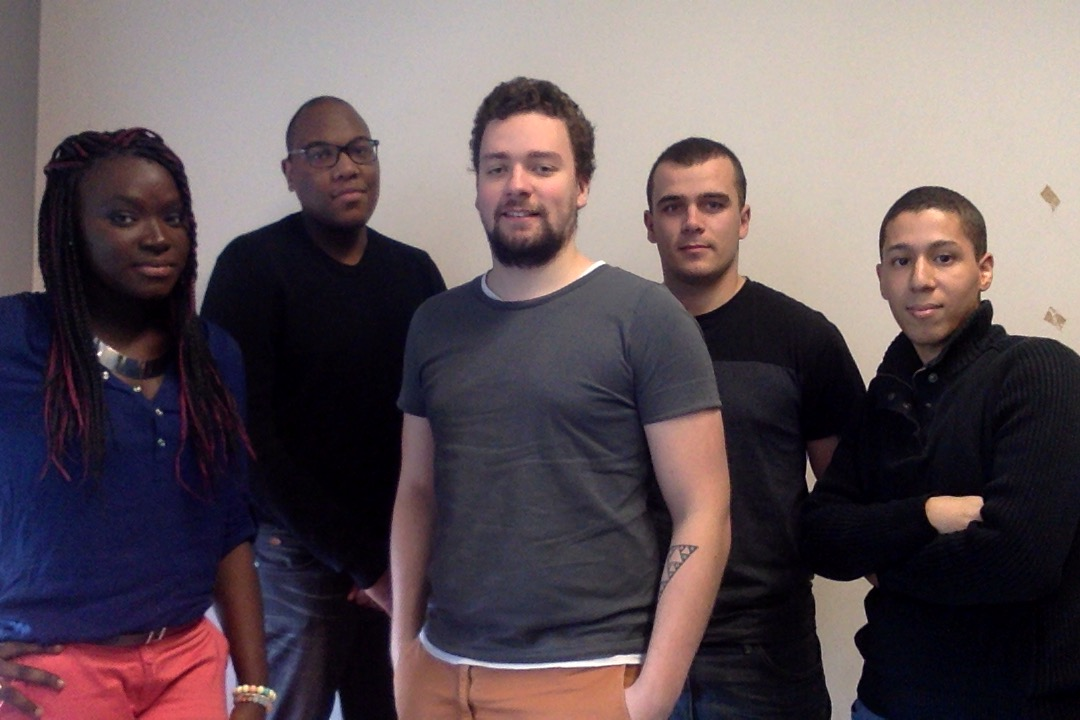
\includegraphics[scale=0.26]{../img/paquiteam.jpg}
	\end{center}
\end{frame}


\begin{frame}
\tableofcontents
\end{frame}

\newcommand\largeur{0.15}

\section{Cas d'utilisation}
\subsection{Diagramme des cas d'utilisation}
\begin{frame}{Diagramme des cas d'utilisation}
	\begin{center}	
		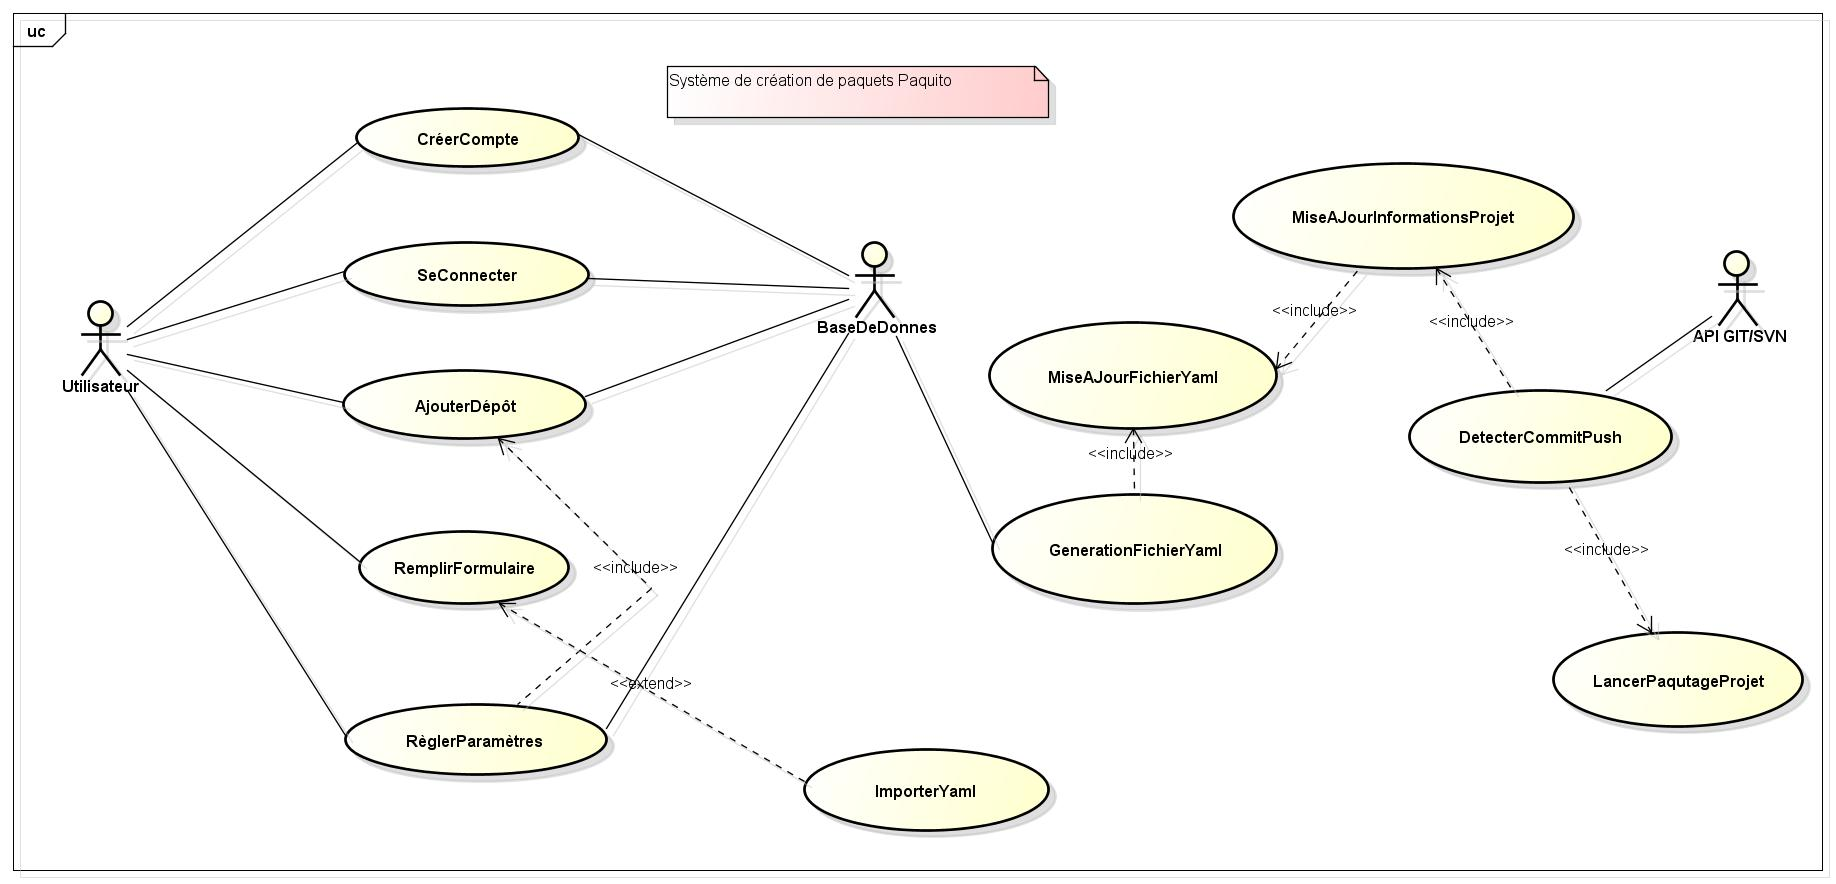
\includegraphics[scale=\largeur]{../img/Diagram1.jpg}
	\end{center}
\end{frame}

\subsection{Détail des cas d'utilisation}
\begin{frame}{Détail des cas d'utilisation}
	\begin{center}	
		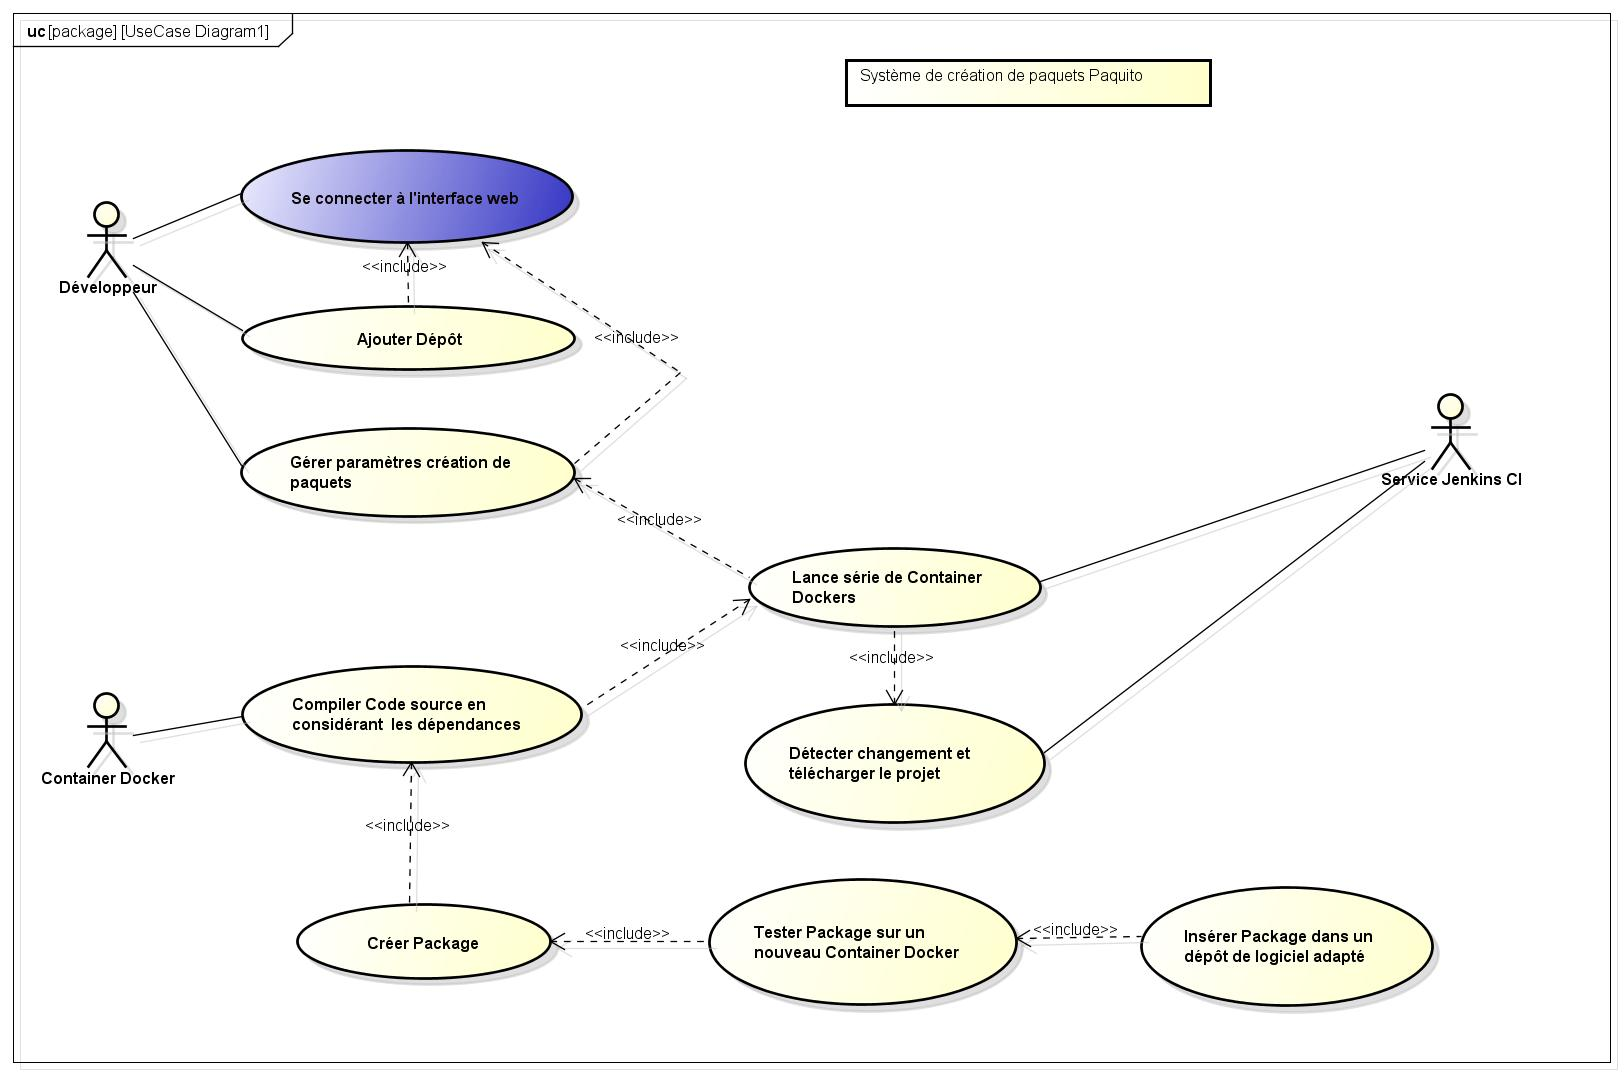
\includegraphics[scale=\largeur]{../img/Diagram2.jpg}
	\end{center}
\end{frame}

\begin{frame}{Détail des cas d'utilisation}
	\begin{center}	
		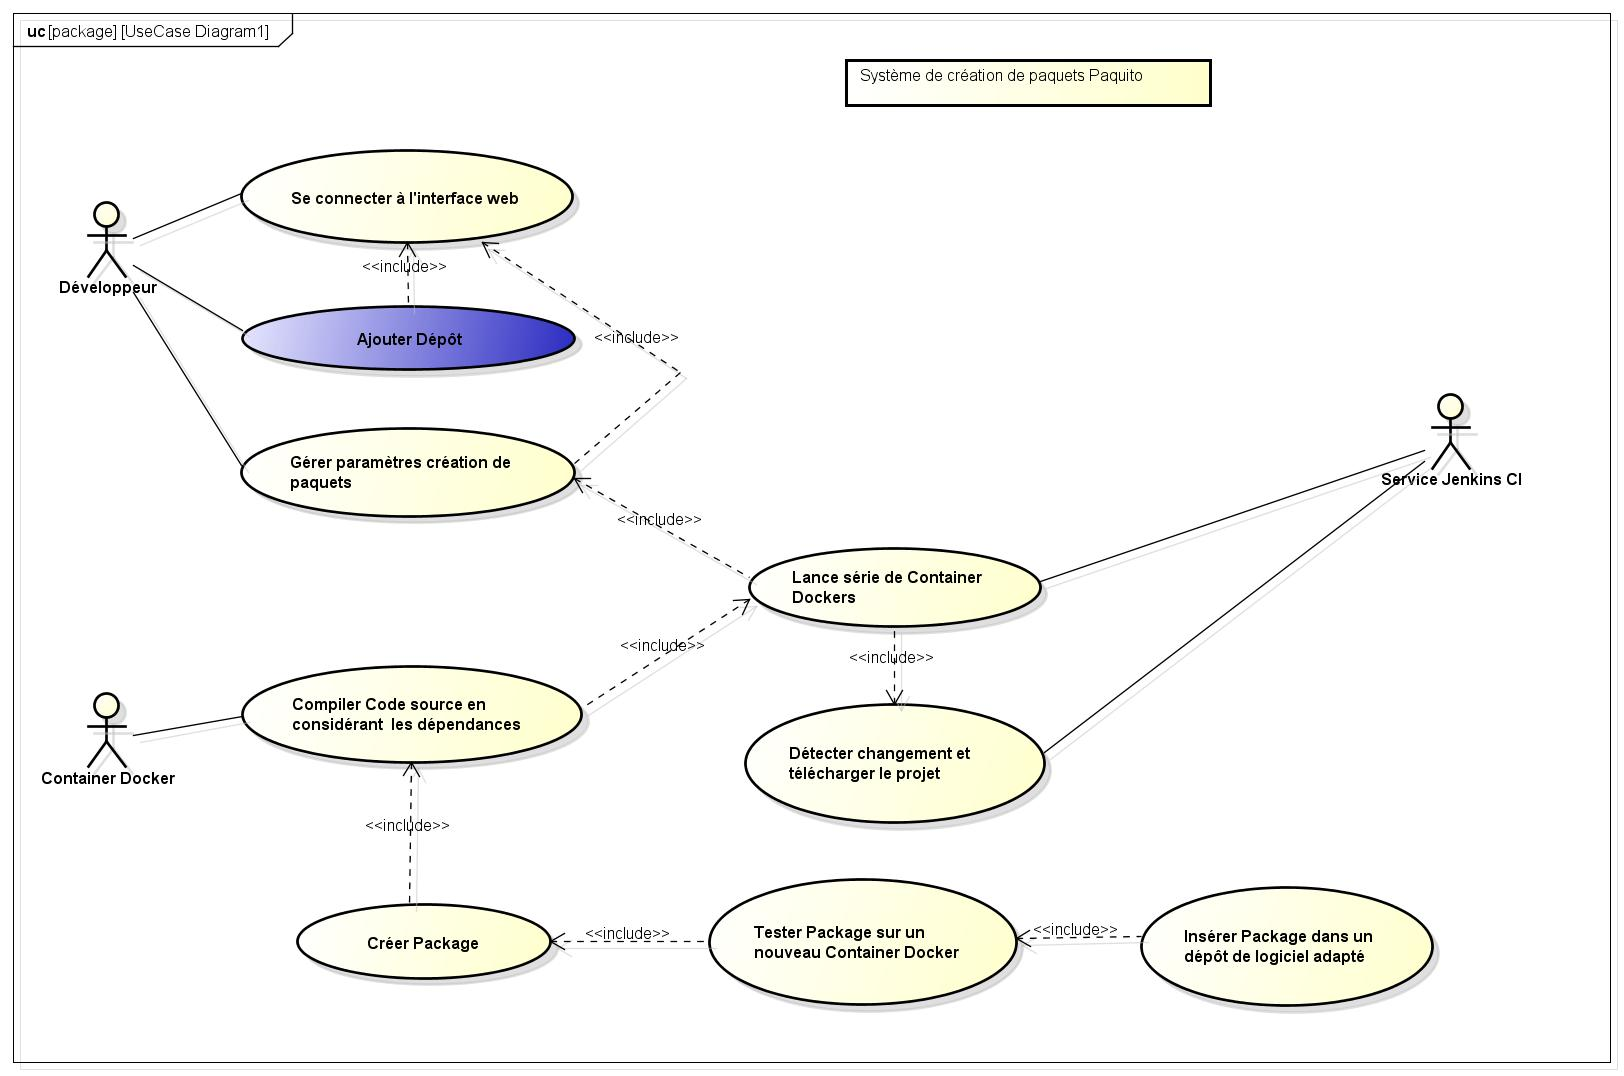
\includegraphics[scale=\largeur]{../img/Diagram3.jpg}
	\end{center}
\end{frame}

\begin{frame}{Détail des cas d'utilisation}
	\begin{center}	
		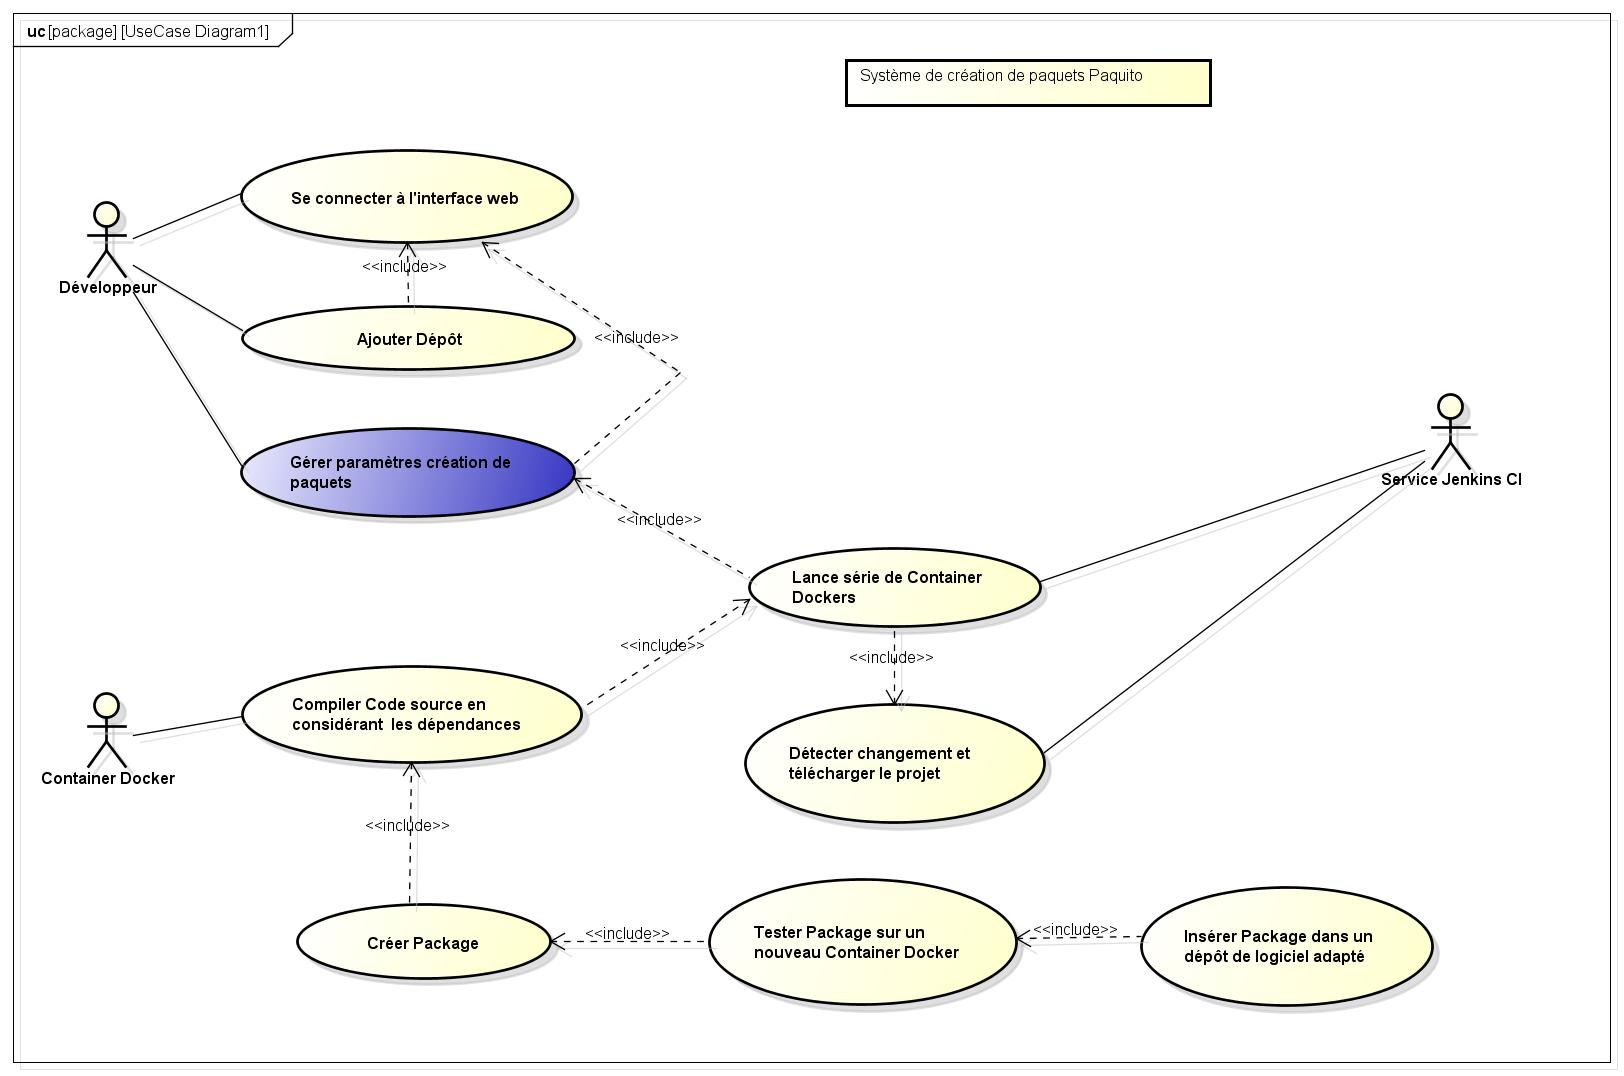
\includegraphics[scale=\largeur]{../img/Diagram4.jpg}
	\end{center}
\end{frame}

\begin{frame}{Détail des cas d'utilisation}
	\begin{center}	
		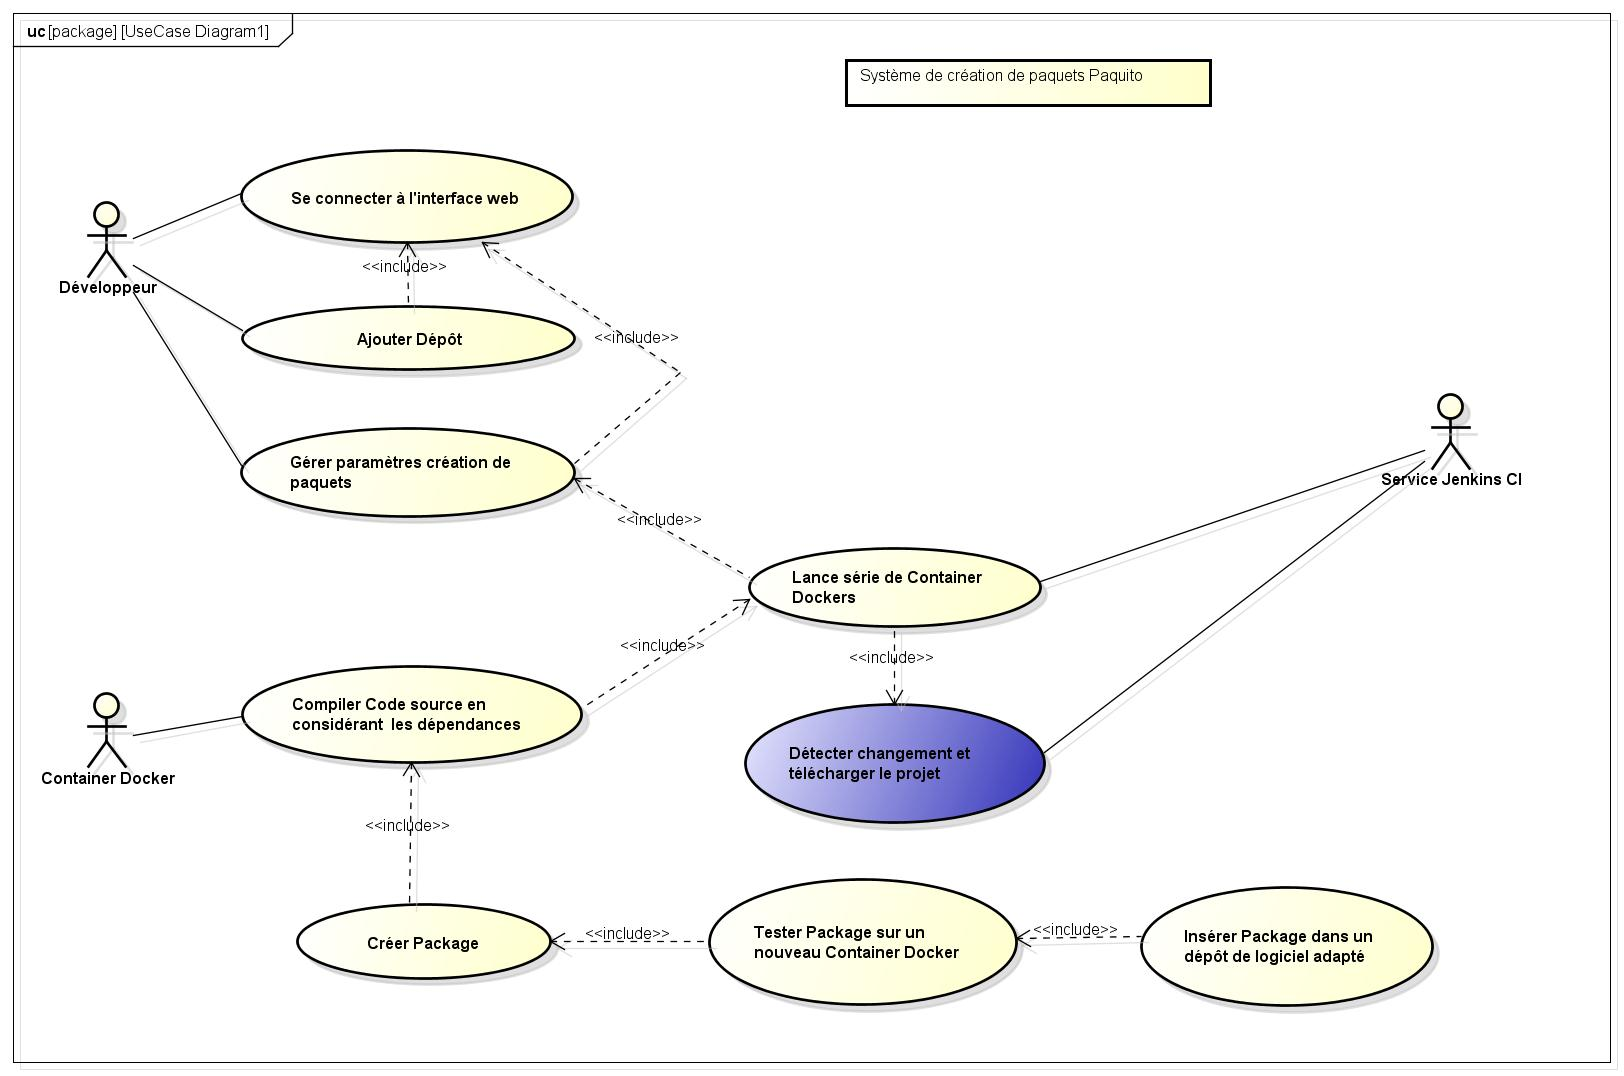
\includegraphics[scale=\largeur]{../img/Diagram5.jpg}
	\end{center}
\end{frame}

\begin{frame}{Détail des cas d'utilisation}
	\begin{center}	
		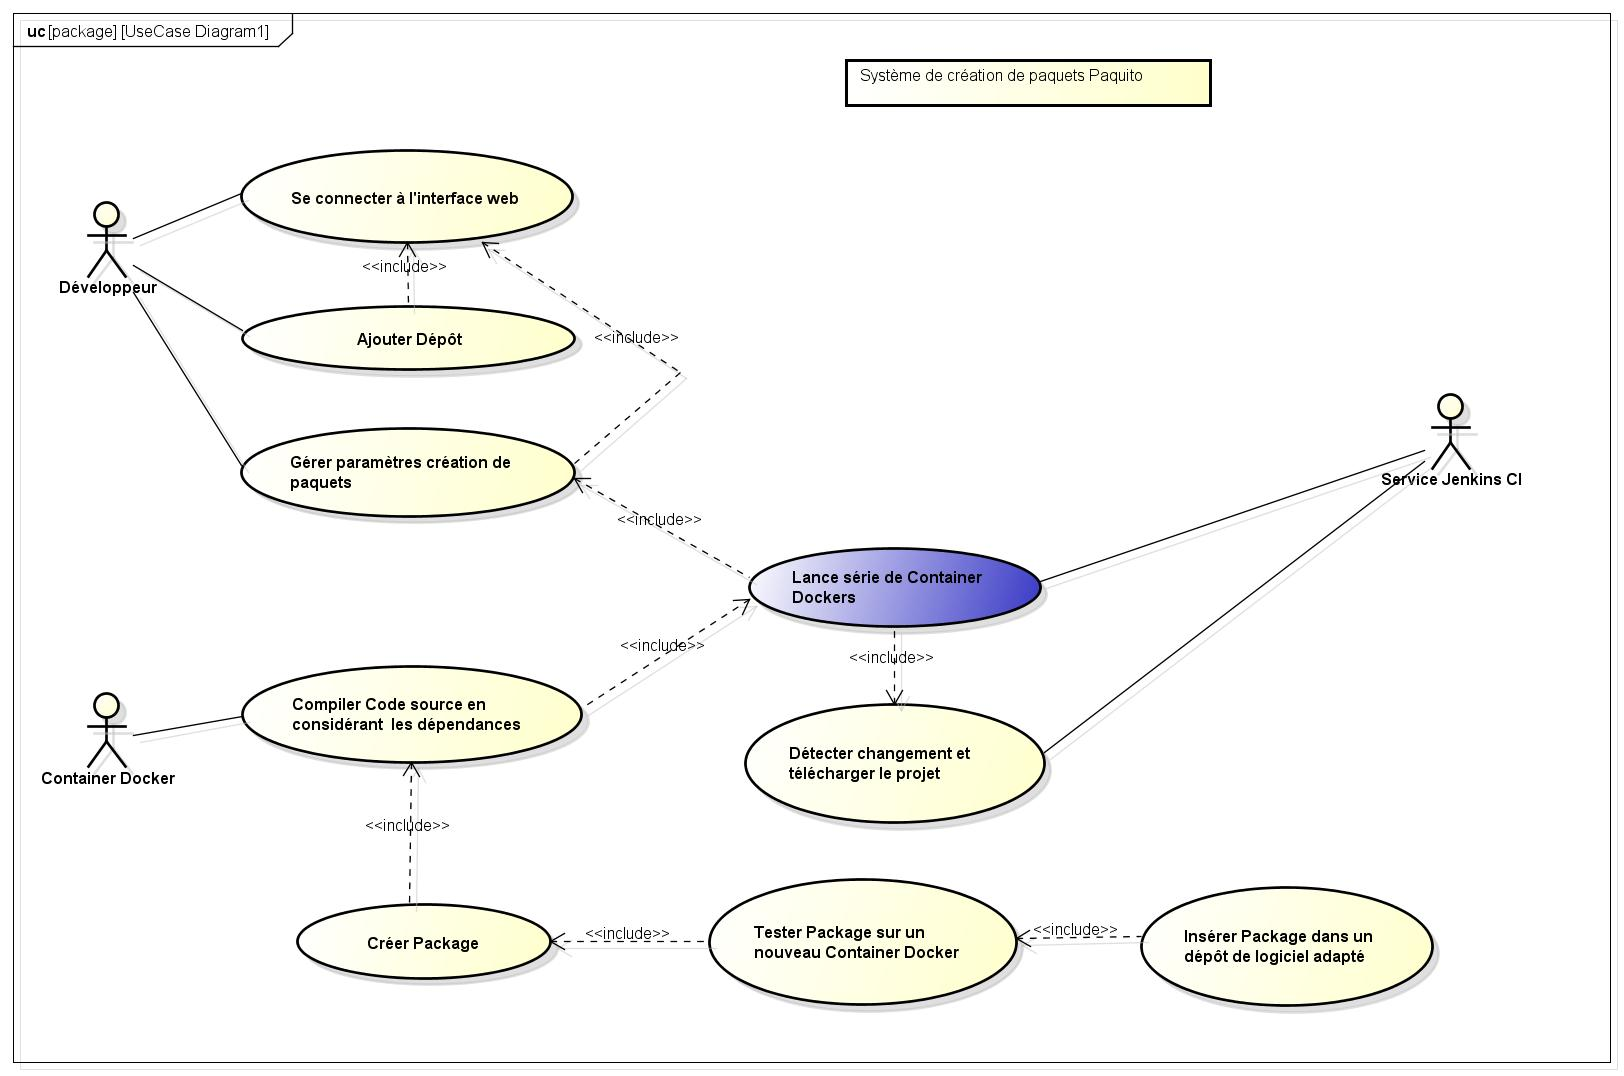
\includegraphics[scale=\largeur]{../img/Diagram6.jpg}
	\end{center}
\end{frame}

\begin{frame}{Détail des cas d'utilisation}
	\begin{center}	
		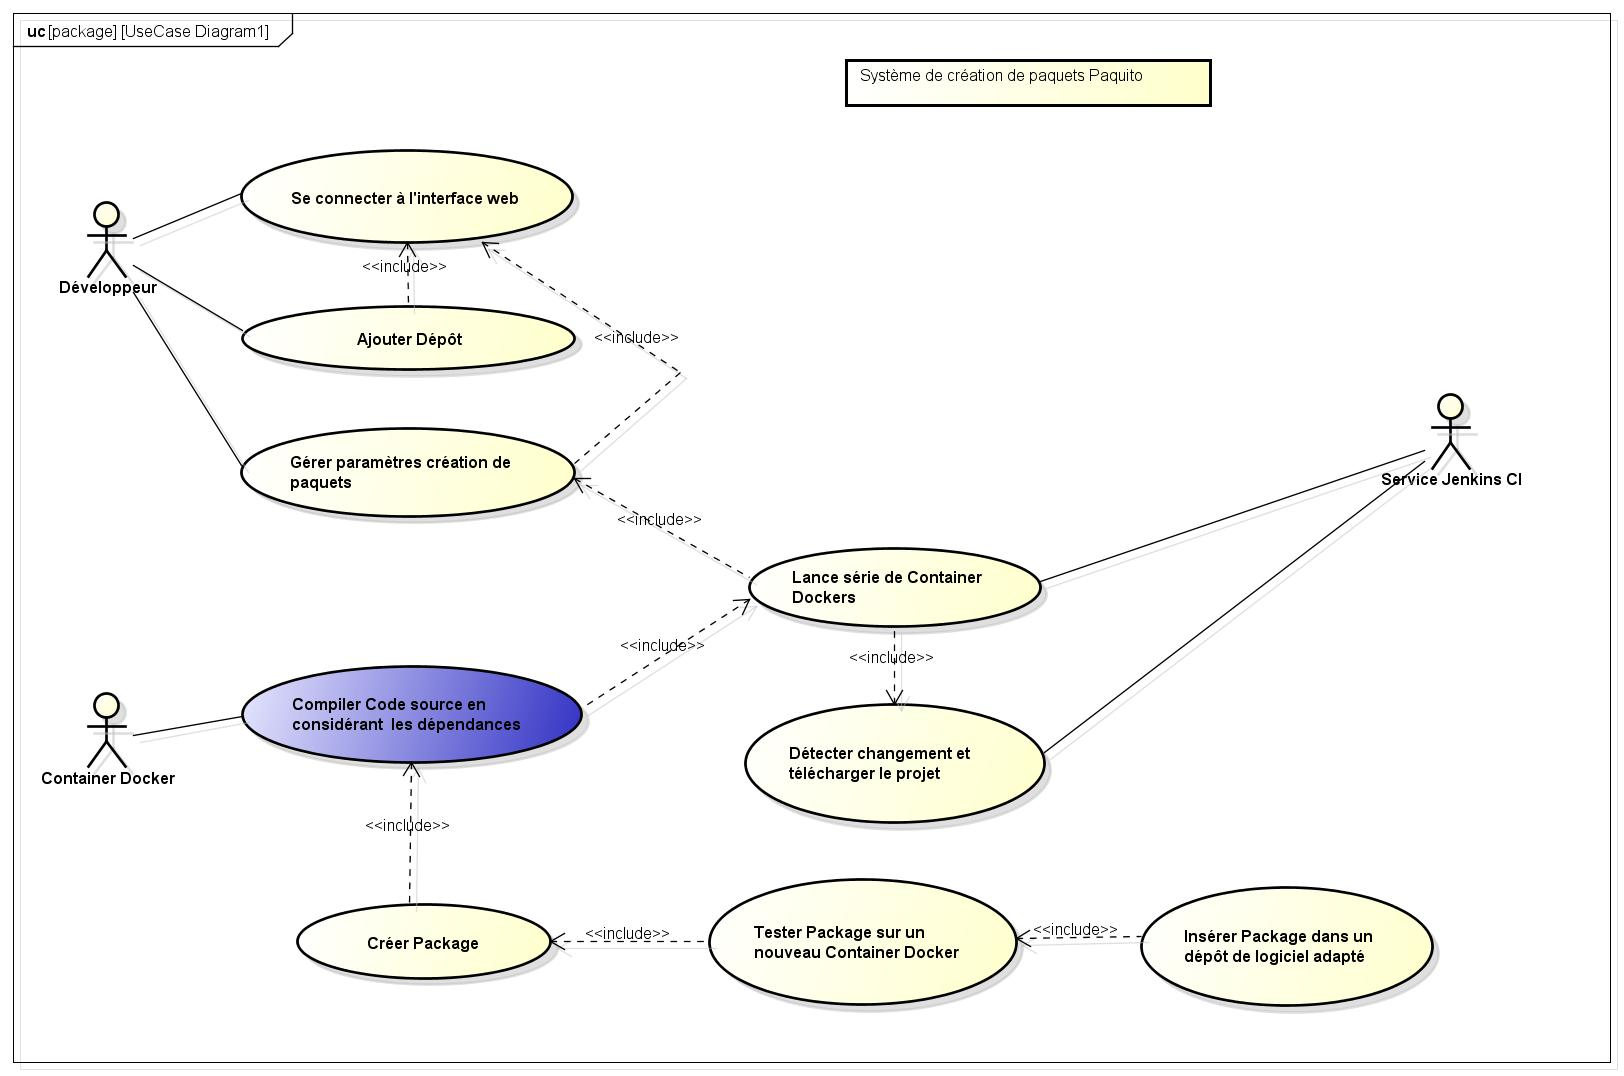
\includegraphics[scale=\largeur]{../img/Diagram7.jpg}
	\end{center}
\end{frame}

\begin{frame}{Détail des cas d'utilisation}
	\begin{center}	
		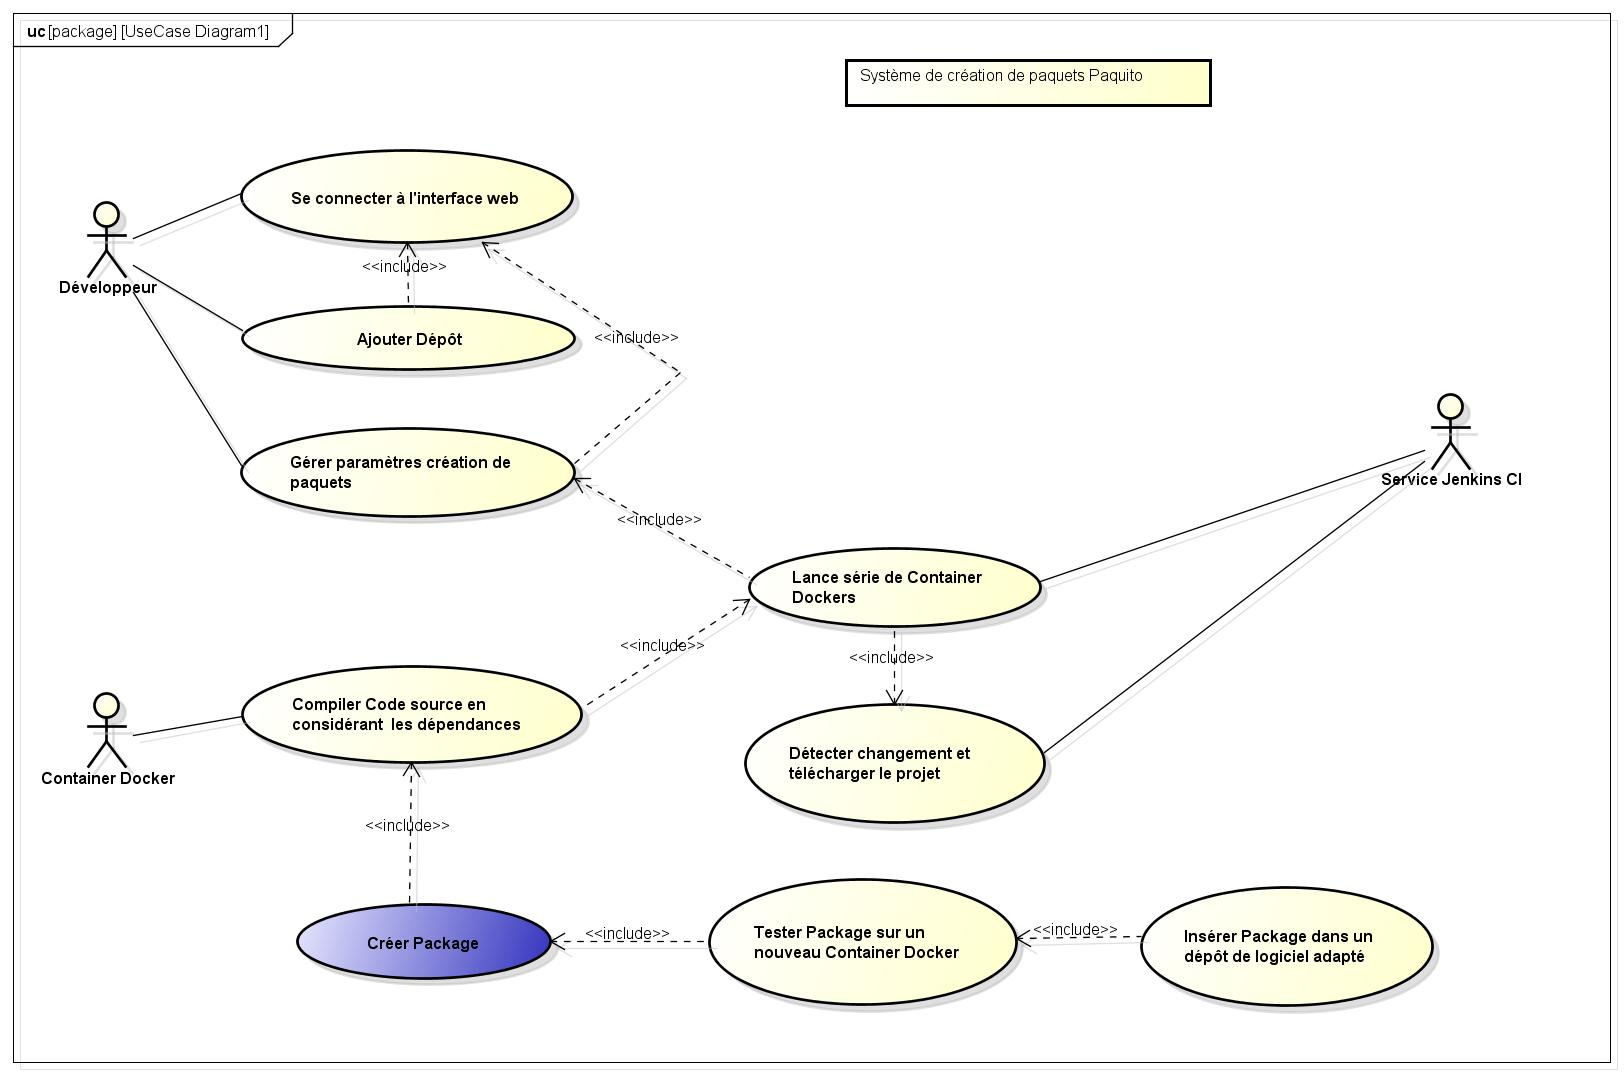
\includegraphics[scale=\largeur]{../img/Diagram8.jpg}
	\end{center}
\end{frame}

\begin{frame}{Détail des cas d'utilisation}
	\begin{center}	
		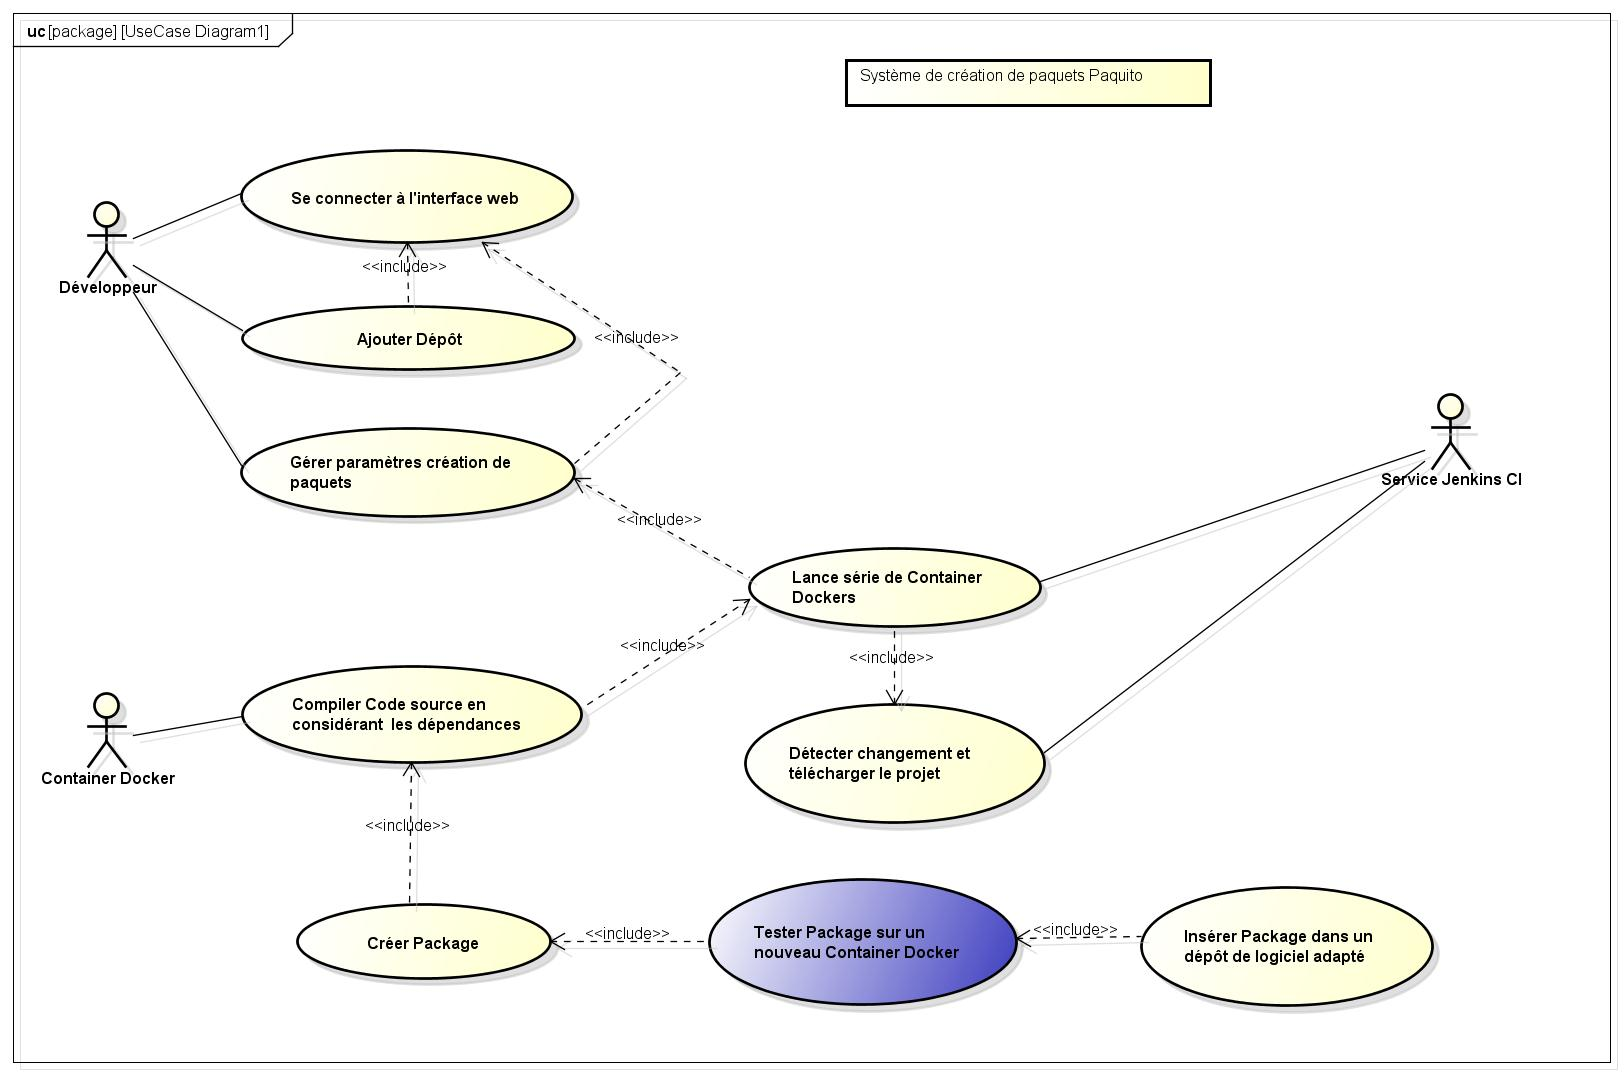
\includegraphics[scale=\largeur]{../img/Diagram9.jpg}
	\end{center}
\end{frame}

\begin{frame}{Détail des cas d'utilisation}
	\begin{center}	
		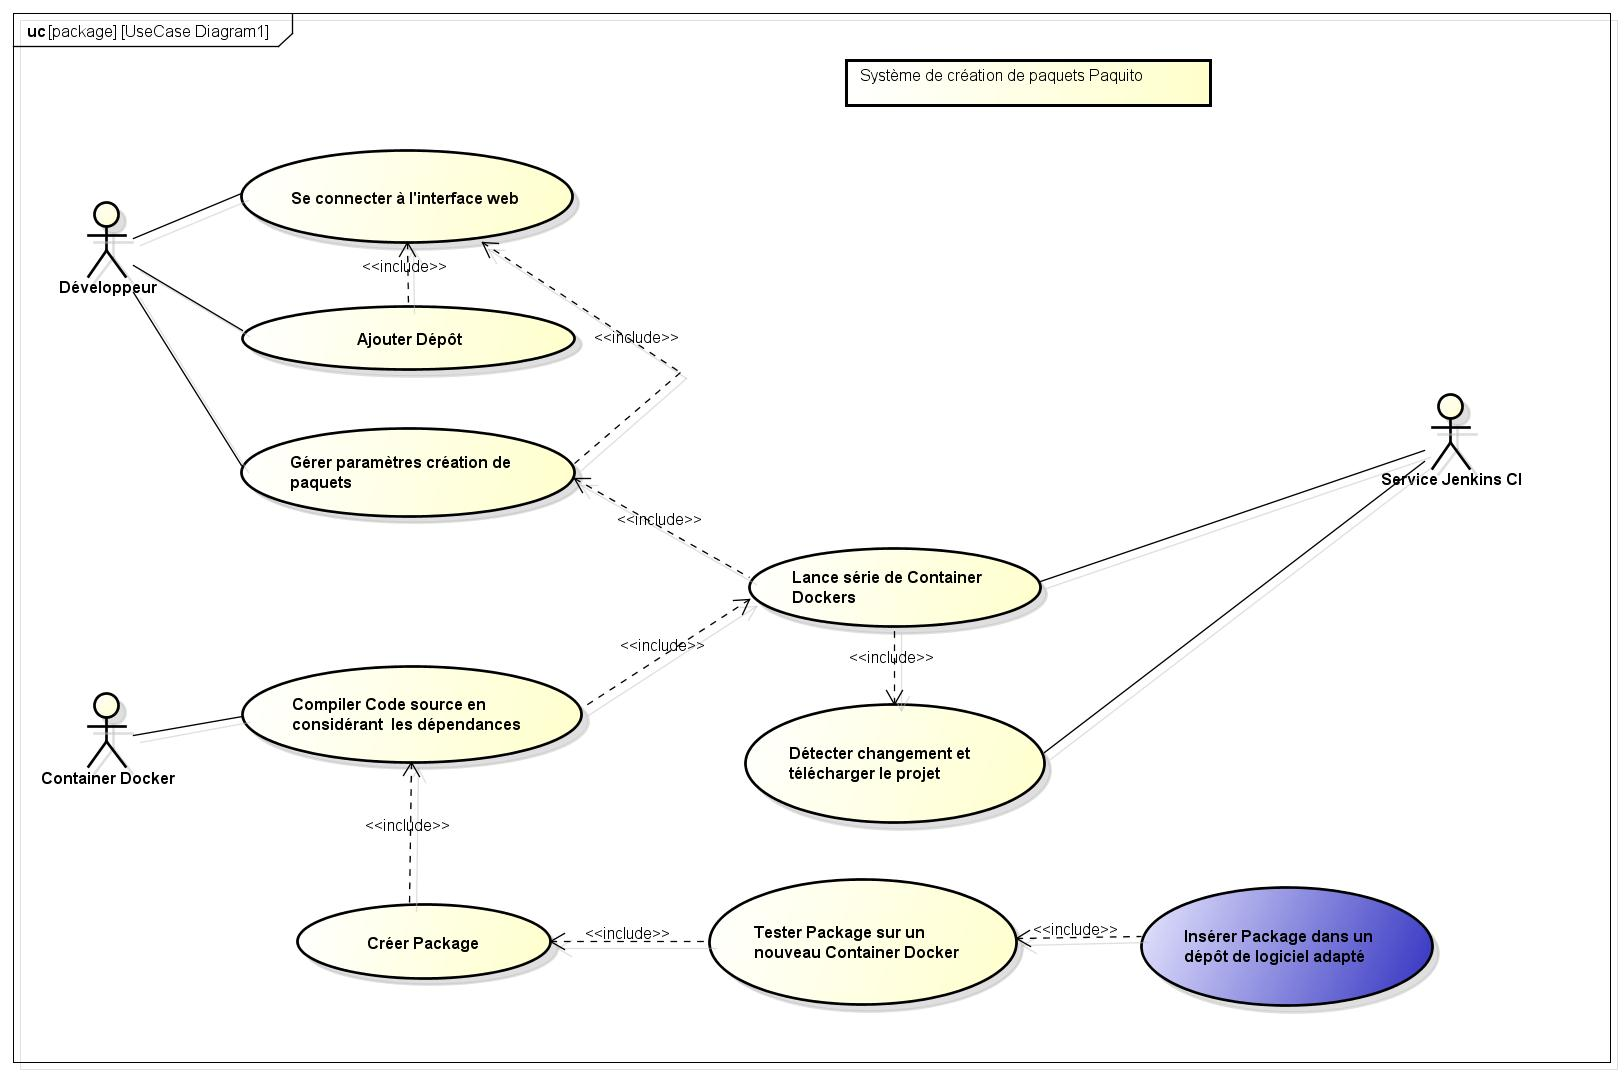
\includegraphics[scale=\largeur]{../img/Diagram10.jpg}
	\end{center}
\end{frame}

\renewcommand\largeur{0.485}

\section{Interface web}
\begin{frame}{Page de connexion et d'inscription}
	\begin{center}
		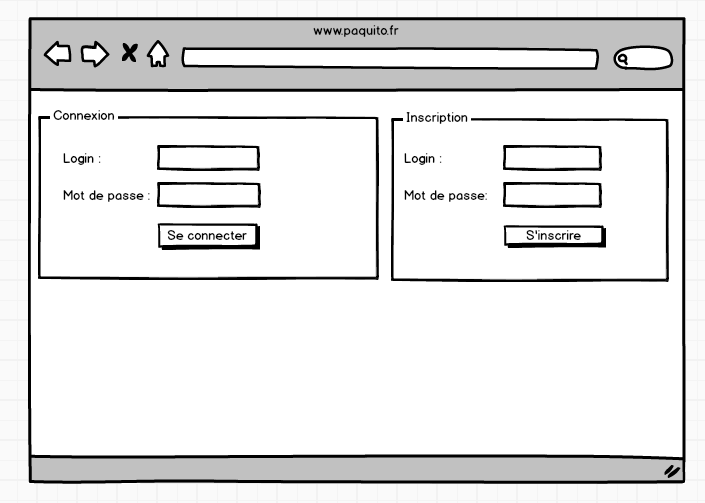
\includegraphics[scale=\largeur]{../img/maquette_1.png}
	\end{center}
\end{frame}

\begin{frame}{Page d'ajout d'un projet à Paquito}
	\begin{center}
		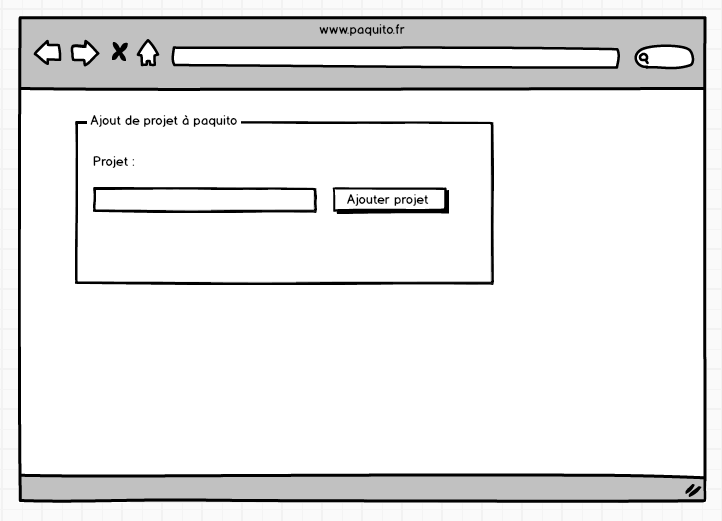
\includegraphics[scale=\largeur]{../img/maquette_2.png}
	\end{center}
\end{frame}

\begin{frame}{Page de résumé d'un projet}
	\begin{center}
		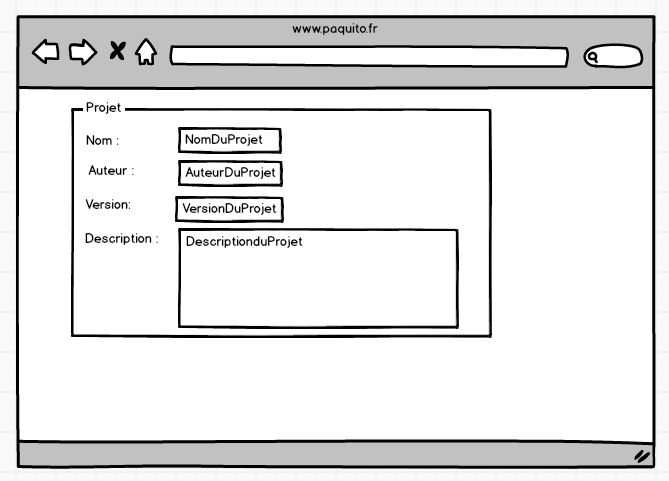
\includegraphics[scale=\largeur]{../img/maquette_3.png}
	\end{center}
\end{frame}


\section*{Conclusion}
\begin{frame}{Conclusion}
	\begin{center}
		
\includegraphics[scale=0.1]{../img/paquito.png}
	
		Merci de nous avoir écouté. 

	\end{center}
\end{frame}

\end{document}